\documentclass[conference]{IEEEtran}

\makeatletter
\newcommand{\rmnum}[1]{\romannumeral #1}
\newcommand{\Rmnum}[1]{\expandafter\@slowromancap\romannumeral #1@}
\makeatother

\usepackage{cite}
\usepackage{amsmath}
\usepackage{amsthm}

\newtheorem{theorem}{Theorem}
\newtheorem{lemma}[theorem]{Lemma}

\ifCLASSINFOpdf
   \usepackage[pdftex]{graphicx}
  % declare the path(s) where your graphic files are
   \graphicspath{{./png/}}
  % and their extensions so you won't have to specify these with
  % every instance of \includegraphics
   \DeclareGraphicsExtensions{.pdf,.png}
\else
  % or other class option (dvipsone, dvipdf, if not using dvips). graphicx
  % will default to the driver specified in the system graphics.cfg if no
  % driver is specified.
  % \usepackage[dvips]{graphicx}
  % declare the path(s) where your graphic files are
  % \graphicspath{{../eps/}}
  % and their extensions so you won't have to specify these with
  % every instance of \includegraphics
  % \DeclareGraphicsExtensions{.eps}
\fi

\ifCLASSOPTIONcompsoc
    \usepackage[caption=false,font=normalsize,labelfont=sf,textfont=sf]{subfig}
\else
    \usepackage[caption=false,font=footnotesize]{subfig}
\fi



% correct bad hyphenation here
\hyphenation{op-tical net-works semi-conduc-tor}
\newcommand{\ignore}[1]{{}}

\begin{document}

\title{Robust Energy-Aware Routing with Uncertain Traffic Demands}


\author{\IEEEauthorblockN{Heng Lin}
\IEEEauthorblockA{Tsinghua University \\ henglin1991@gmail.com}
\and
\IEEEauthorblockN{Mingwei Xu}
\IEEEauthorblockA{Tsinghua University \\ xmw@cernet.edu.cn}
\and
\IEEEauthorblockN{Yuan Yang}
\IEEEauthorblockA{Tsinghua University \\ yyang@csnet1.cs.tsinghua.edu.cn}}


% make the title area
\maketitle

% As a general rule, do not put math, special symbols or citations
% in the abstract
\begin{abstract}
Energy conservation has become a major challenge to the Internet. In existing approaches, a part of line cards
are switched into sleep mode for energy conservation, and the routing is configured carefully to balance energy saving
and traffic engineering goals, such as the maximum link utilization ratio (MLUR). Typically, traffic demands are
used as inputs, and routing is computed accordingly. However, accurate traffic matrices are difficult to obtain and
are changing frequently. This makes the approaches difficult to implement. Further, the routing may shift
frequently, and is not robust to sudden traffic changes.

In this paper, we propose a different approach that finds one energy-aware routing robust to a set of traffic
matrices, particularly to arbitrary traffic demands. Such a routing without energy consideration is known as
the demand-oblivious routing, and is well studied. However, the problem becomes much more challenging when energy
conservation is involved. To overcome the challenges, we first define a new metric, namely oblivious performance
ratio with energy constraint (OPRE), which reflects the MLUR distance from a routing to the optimal routing when
certain energy conservation requirement is satisfied. We model the problem of minimizing the performance ratio,
and analyze the lower and the upper bounds. Then, we propose Robust Energy-Aware Routing (REAR) to solve
the problem in two phases. REAR select sleeping links based on extended robust link utilization (ERLU)
and compute the routing based on a classical demand-oblivious routing algorithm.
We evaluate our algorithms on real and synthetic topologies. The simulation results show that REAR can save
19\% of line card power while the performance ratio is less than 34\%.
\end{abstract}

\IEEEpeerreviewmaketitle

\section{Introduction}
\label{introduction}

Energy conservation has become a global concern nowadays. The Internet is one of the major energy consumers, and its rapid growth makes the green Internet a hot research topic. In the Internet backbone, energy is mainly drawn by routers and switches. Such devices consume almost full power even if the traffic load is small. Thus, an effective method to save energy in the Internet is to aggregate traffic into part of the routers when the traffic load is small, and switch the under-utilized components (routers or line cards) into off/sleep mode. Such a method is known as the energy efficient routing.

An important issue for energy efficient routing is to avoid network congestion after the traffic is aggregated. Many approaches have been proposed in existing works. Most approaches compute the routing based on real-time traffic matrices or link loads, to achieve a good load balancing and avoid congestion. However, such approaches come at a cost of obtaining real-time traffic data. Furthermore, the routing may shift frequently with the traffic changes, and a sudden traffic change may still induce congestions. To this end, we need to study the robustness of energy efficient routing.

Specifically, we study the energy efficient routing when traffic matrices cannot be obtained or predicted precisely, i.e., with uncertain traffic demands. To achieve robustness, we need to find a routing, which can perform near optimally under a range of traffic matrices. The key technique that makes this possible is the advanced \emph{demand-oblivious routing}. A seminal work \cite{networking:oblivious} find that, the distance between the maximum link utilization ratio (MLUR) of a demand-oblivious routing and the MLUR of the optimal routing is bounded. Thus, no matter how the traffic demand changes, the demand-oblivious routing can guarantee certain performance. We note that this conclusion is in a network without sleeping components, and we need to consider the situation when energy conservation is required.

However, existing demand-oblivious routing algorithms cannot be directly applied to energy efficient routing. There are several challenges. First, we need to define a metric that can effectively measure the distance between a robust energy efficient routing and the optimal routing, because the existing metric for demand-oblivious routing fails in the situation when some components are switched into off/sleep mode. Second, we need to analyze whether the metric can be bounded, just like for demand-oblivious routing. If there exists no bound, then it is not feasible to find a robust energy efficient routing. Third, we need practical algorithms to compute the robust energy efficient routing. Specifically, we need to determine: 1) which routers or line cards should be switched into off/sleep mode, to achieve energy efficiency; and 2) in which path to forward the traffic for robustness, while the path does not traverse the sleeping components.

In this paper, we overcome the aforementioned challenges. First, we define a new metric, namely the oblivious performance ratio with energy constraint (OPRE). The OPRE reflects the MLUR distance from a routing to the optimal one when certain energy conservation requirement is satisfied. We model the problem of minimizing the OPRE. Second, we prove that there exists a robust energy efficient routing with the minimum OPRE, which has an upper bound given a network. Then, we propose Robust Energy-Aware Routing (REAR) scheme, which uses heuristic algorithms to solve the problem. We develop algorithm RLP, which chooses sleeping line cards in a way that the OPRE can be minimized potentially. We then develop algorithm RRA to compute the routing in the remaining topology, by extending existing optimal demand-oblivious routing algorithm. We evaluate our algorithms by simulations on real topologies and synthetic traffic demands with random fluctuations. The results show that REAR can achieve an OPRE of 1.34 while 19\% of line card power is saved.

The rest of the paper is organized as follows. Section \ref{related_work} shows the related work. Section \ref{problem_statement} presents metric OPRE and formally models the problem. We presents the bounds on OPRE in Section \ref{upper_bounds_of_the_minimum_opre}, and propose our algorithms in Section \ref{robust_energy_aware_routing_algorithms}. Section \ref{performance_evaluation} shows our simulation setup and results, and Section \ref{conclusion} concludes our work.


\section{Related Work}
\label{related_work}
Green routing is studied because we can not use as much of a resource as we need \cite{networking:designing}, such as line cards always work in full mode even with 
low traffic fraction. So there are many studies to save energy consumption by put some links in sleep mode, for example GreenTE \cite{networking:greente} is 
proposed for maximuming the sleeping links while $E^2$-MCRA \cite{networking:active} is proposed for minimizing the active links and nodes by a depth-first search approach.
Besides these centralized algorithms, EAR \cite{networking:car} and GRiDA \cite{networking:grida} are proposed for distributed deployment, both of them are compatible 
with OSPF sharing additional information between nodes. For addressing the problem of routing convergence when traffic changes frequently, GreenFRR 
\cite{networking:greenfrr} is proposed by leveraging the technique of fast rerouting.

Network may suffer from bad performance because of both frequent traffic demand and routing changes. There are studies to estimate traffic matrices in the context
of Internet traffic, such as LP approach \cite{networking:lp}, Bayesian Infereence techniques \cite{networking:bayesian} and Time-Varying Network Tomography
\cite{networking:time}. All the estimatation for traffic matrices result in the changes of routing, \cite{networking:minimize} proposed an oblivious routing algorithm with a polylog 
competitive ratio with respect to congestion and \cite{networking:polynomial} give a polynomial time algorithm based on applying the Ellipsoid algorithm to an exponential-size LP model.
To be practical for large networks, the oblivious-demand routing based on polynomial-size LP formulation is investigated in \cite{networking:oblivious}.

In this paper, we proposed robust energy-aware routing based on the oblivious-demand \cite{networking:oblivious}, which is both green for the energy consumption by pruning
some links based on ERLU, and also robust for uncertain traffic demands. It is more practical than existing green routing algorihtm because it almost do not need changes when 
real traffic varifies.


\section{Problem Statement}
\label{problem_statement}

\subsection{Background of Demand-Oblivious Routing}

As mentioned above, demand-oblivious routing aims at finding one routing that performs near optimally under a range of traffic demands. In traffic engineering, a typical metric to evaluate routing performance is the maximum link utilization ratio (MLUR). Clearly, the MLUR is corresponded with a specified traffic matrix (TM). Demand-oblivious routing defines oblivious performance ratio (OPR) to evaluate the routing performance without the knowledge of TM. We briefly present the background.

Given a TM, the distance between a routing to the optimal one is defined as the ratio between their MLURs. Formally, a network is modeled as undirected graph $G(V, E)$, where $V$ is the set of vertices (nodes), and $E$ is the set of edges (links). Let $cap_{ij}$ denote the capacity of the link $(i, j) \in E$. Let $d_{ab}$ denote the traffic demand from origin node $a$ and destination node $b$, and $m$ denote the TM that contains $d_{ab}$ for all $a, b \in V$. Let $f^r_{ab}(i,j)$ be the fraction of $d_{ab}$ that is routed on link $(i, j)$ $(0 \leq f^r_{ab}(i,j) \leq 1)$, using routing $r$. Routing $r$ is specified by $f^r_{ab}(i,j)$ for all $a, b \in V$ and $(i, j) \in E$, and we will formally define routing consistency later in Section III.C. Let $U_{r, m, G}$ be the MLUR of routing $r$ under TM $m$. We have

\begin{equation}
\label{equation_U_rmG}
	U_{r, m, G} = \max_{(i,j)\in E} \frac{\sum_{a,b} d_{ab}f^r_{ab}(i,j)}{cap_{ij}}.
\end{equation}

Let $P(\{ r \},\{ m \}, G)$ be the \emph{performance ratio} of routing $r$ under TM $m$, which reflects how far from the routing to the optimal one, and is defined as
\begin{equation}
\label{equation_P_rmG}
	P(r,\{ m \}, G) = \frac{U_{r,m,G}}{\min_{r'} U_{r', m, G}}.
\end{equation}

The \emph{oblivious performance ratio} (OPR) for routing $r$ is defined by extending TM $m$ to a set of TMs $M$, where $M$ can be the set of all TMs. We have
\begin{equation}
\label{equation_P_rMG}
	P(r, M, G) = \max_{m\in M} P(r, \{ m \}, G).
\end{equation}
The target of demand-oblivious routing is to find routing $r$ that minimizes OPR $P(\{ r \}, M, G)$. Such a ``robust'' routing is independent of a specific TM, but can perform near optimally. A seminal work \cite{networking:oblivious} uses linear programming to find the routing that minimizes the OPR, and finds that the optimal solution exists, which means that the OPR is bounded.

\subsection{Oblivious Performance Ratio with Energy Constraint}

With energy constraint, a network may have to switch part of line cards into off/sleep mode to save the total energy consumption. This changes the network topology and makes metric OPR fail to evaluate the robustness of a routing. We use an example to show this. Assume that $G$ is a cycle with $n$ unit capacity links. Then, the minimal OPR of $G$ is $2-2/n$ \cite{networking:oblivious}. Now we pruning one link from $G$ to save energy, and the topology changes to $G^*$. Because there is only one routing feasible in $G^*$, OPR $P(\{ r \}, M, G^*)$ equals 1. Since 1 is less than $2-2/n$ for $n > 2$, it means that the routing after pruning one link is more robust than before. However, it is false because there are less links and the network is more likely to be congested.

The intrinsic reason for such a ``fake robust'' is that the topology is not changing when performance ratio is computed in Eq. (\ref{equation_P_rmG}). To address this issue, we extend the definition of OPR. Formally, let $G^*$ be a sub-graph of $G$ that satisfies the energy constraint (We will formally define the energy constraint in Section III.C, i.e., Eq. (\ref{inequation_power_threshold})). Note that in this case, a path cannot traverse a sleeping link, so routing $r$ is limited by $G^*$ (Eq. (\ref{equation_flow_for_routing}) in Section III.C). The extended performance ratio is defined as
\begin{equation}
\label{equation_P_rmGG}
	P(r, \{ m \}, G, G^*) = \frac{U_{r,m,G^*}}{\min_{r'} U_{r', m, G}}.
\end{equation}
Let $P^*(r, M, G, G^*)$ be the \emph{oblivious performance ratio with energy constraint} (OPRE) for routing $r$. We define $P^*(r, M, G, G^*)$ by extending $m$ to $M$. Similar to Eq. (\ref{equation_P_rMG}), we have
\begin{equation}
\label{equation_P_rMGG}
	P^*(r, M, G, G^*) = \max_{m\in M} P(r, \{ m \}, G, G^*).
\end{equation}
Note that $G^*$ is used to achieve certain energy conservation target. For an energy conservation target, there may exist a set of different $G^*$, which result in different OPRE. We will show an example below. When there is no energy constraint, $G^*$ equals $G$, and Eq. (\ref{equation_P_rMGG}) naturally reduces to Eq. (\ref{equation_P_rMG}).

\subsection{Example}

We show an example of our new metric OPRE. The network is shown in Fig. \ref{figure_an_example_of_opre}, where two nodes $a, b$ are connected by two links $l_1$ and $l_2$.{\footnote{When there are parallel links, we can add a virtual node in each parallel link to keep $G(V,E)$ as a simple graph.}} The capacities of the links are 3 Mbps and 4 Mbps, respectively. To forward a traffic demand of $d_{ab}$, the optimal routing is to put $\frac{3}{7}d_{ab}$ on link $l_1$ and $\frac{4}{7}d_{ab}$ on link $l_2$, which results in the MLUR of $\frac{1}{7}d_{ab}$. This routing is also the optimal demand-oblivious routing, because the routing is optimal no matter how $d_{ab}$ changes. Thus, the OPR equals 1.

\begin{figure}[!t]
\centering
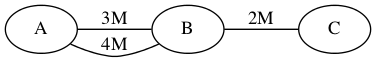
\includegraphics[width=1.3in]{3-nodes-example}
\vspace{-0.15in}
\caption{An example of the OPRE, where the traffic demand is $d_{ab}$.}
\label{figure_an_example_of_opre}
\end{figure}

Now, assume that links $l_1$ and $l_2$ consume the same power, and one link has to be switched off/sleep to save energy. Let us check the OPRE after pruning $l_1$ and $l_2$, respectively. If $l_1$ is pruned, $d_{ab}$ is put on link $l_2$, and the MLUR is $\frac{1}{4}d_{ab}$, so the OPRE is $\frac{1}{4}d_{ab}/\frac{1}{7}d_{ab} = 7/4 = 1.75$. If $l_2$ is pruned, $d_{ab}$ traverses link $l_1$, resulting in the MLUR of $\frac{1}{3}d_{ab}$, so the OPRE is $\frac{1}{3}d_{ab}/\frac{1}{7}d_{ab} = 7/3 = 2.33$. The results tell us that pruning link $l_1$ is more robust than pruning link $l_2$. This is consistent with the intuition that link $l_2$ has a larger capacity and is stronger against congestion.

\subsection{Problem Formulation}

Now we formally model the problem. Our objective is to minimize OPRE $P^*(r, M, G, G^*)$, where $M$ and $G$ are inputs, and routing $r$ and sub-graph $G^*$ are decision variables. The Min-OPRE problem is as follows.

\begin{center}
Minimize \quad $P^*(r, M, G, G^*)$
\end{center}

\begin{center}
s.t. (1),\ (4),\ (5)
\end{center}

\begin{center}
    $\forall a,b,i \in V$: \quad \quad \quad \quad \quad \quad \quad \quad \quad \quad \quad \quad \quad \quad \quad
    \vspace{-0.3in}
\end{center}

\begin{equation}
\label{equation_flow_for_routing_second}
    \begin{split}
    \sum_{j, s.t.(i,j) \in E}\hspace{-0.2in}f^{r'}_{ab}(i,j) - \hspace{-0.2in}\sum_{j, s.t.(j,i) \in E}\hspace{-0.2in}f^{r'}_{ab}(j,i) =
    \left\{
        \begin{array}{c}
        \ \ 1, \ i = a \\
        -1, \ i = b \\
        \ \ \ \ \ 0, \ i \neq a,b \\
        \end{array}
    \right.
    \end{split}
\end{equation}

\begin{center}
    \vspace{0.1in}
    $\forall a,b,i \in V$: \quad \quad \quad \quad \quad \quad \quad \quad \quad \quad \quad \quad \quad \quad \quad
    \vspace{-0.3in}
\end{center}

\begin{equation}
\label{equation_flow_for_routing}
    \begin{split}
    \sum_{j, s.t.(i,j) \in E^*}\hspace{-0.2in}f^r_{ab}(i,j) - \hspace{-0.3in}\sum_{j, s.t.(j,i) \in E^*}\hspace{-0.2in}f^r_{ab}(j,i) =
    \left\{
        \begin{array}{c}
        \ \ 1, \ i = a \\
        -1, \ i = b \\
        \ \ \ \ \ 0, \ i \neq a,b \\
        \end{array}
    \right.
    \end{split}
\end{equation}

\begin{center}
    \vspace{0.1in}
    $\forall a,b \in V$, $\forall i,j \in E$: \quad \quad \quad \quad \quad \quad \quad \quad \quad \quad \quad
    \vspace{-0.15in}
\end{center}

\begin{equation}
\label{inequation_traffic_fraction}
    0 \leq f^r_{ab}(i,j),f^{r'}_{ab}(i,j) \leq 1
\end{equation}

\begin{equation}
\label{inequation_power_threshold}
    \sum_{l \in E^*} p(l) / \sum_{l \in E} p(l) \leq 1 - \theta
\end{equation}

Constraints (\ref{equation_U_rmG}), (\ref{equation_P_rmGG}), and (\ref{equation_P_rMGG}) follow our definition of the OPRE. Eq. (\ref{equation_flow_for_routing_second}) means that the optimal routing $r'$ in $G$ must be a valid routing, i.e. with routing consistency. Specifically, for the source/destination node, all traffic must be routed/received; and for an intermediate node, the traffic flowing out must equal the traffic flowing in. Similarly, Eq. (\ref{equation_flow_for_routing}) means that the robust routing $r$ in $G^*$ must be a valid routing. Ineq. (\ref{inequation_traffic_fraction}) means that the range of $f^r_{ab}(i,j)$ and $f^{r'}_{ab}(i,j)$ is from 0 to 1. Ineq. (\ref{inequation_power_threshold}) means that the power consumption of links in $G^*$ must be less than a given threshold. In Ineq. (\ref{inequation_power_threshold}), $\theta$ denotes the power saving ratio we must achieve by using $G^*$. Here, we use $p(l)$ to denote the power consumption of link $l$, which is mainly drawn by the line cards at the two ends of the link. Note that $p(l)$ is independent of the traffic volume, and this assumption is based on the fact that in current stage, the power of a line card changes little with the traffic volume \cite{networking:hopbyhop}.

Note that if $G^* = G$ satisfy the energy constraint Ineq. (\ref{inequation_power_threshold}) and $M$ is the set of all TMs, the Min-OPRE problem reduces to the demand-oblivious routing problem, and can be transformed into a linear program and solved in polynomial time \cite{networking:oblivious}. However, we must find the optimal $G^*$ to achieve the required power saving ratio in other cases, and Min-OPRE is an MILP and is NP-hard in general.

Also note that we put the power saving in the constraint of our problem, instead of the objective function. In such a way, we can balance the trade off between energy conservation and the OPRE, by setting different values of power saving ratio $\theta$. We can even achieve the maximum power saving ratio by a binary search on $\theta$.

\section{Upper Bounds of the Minimum OPRE}
\label{upper_bounds_of_the_minimum_opre}

In this section, we analyze the upper bounds of the minimum OPRE. We are interested in two extreme types of networks, i.e., cycles and cliques, because general networks can be seen as intermediate cases between them. We will present the upper bounds with small and large values of $\theta$. We find that, though the minimum OPR of cycles and cliques is similar and bounded by 2 \cite{networking:oblivious}, the minimum OPRE is much more different and has a larger upper bound with a larger $\theta$. These theoretical results tell us that the robust energy efficient routing exists, and tell us how close a robust routing can get to the optimal routing.

\begin{lemma}
$\min P^*(r, M, G, G^*) \geq \min P^*(r, M, G)$ if $G^* \subseteq G$, where the equation holds if $G^* = G$.
\end{lemma}
\begin{proof}
We assume exist a $G^*$, s.t. min $P^*(r,M,G,G^*)$ $<$ min $P^*(r, M, G)$. Becuase $G^*$ is the subset of $G$, we directly
use the robust routing of $G^*$ to $G$, then $P^*(r, M, G)$ will equal to $P^*(r,M,G,G^*)$, and arise contradiction.
Particularly, when $G^* = G$, $G^*$ is the subset of $G$, and $G$ is the subset of $G^*$, so there is both
min $P^*(r,M,G,G^*)$ $\geq$ min $P^*(r, M, G)$ and $P^*(r, M ,G)$ $\geq$ $P^*(r, M, G, G^*)$, so they are equal to each other
when $G^*$ = $G$. This ends our proof.
\end{proof}

\begin{theorem}
The minimum OPRE of $C_n$ (the cycle on $n$ vertices with unit capacity links) and $K_n$ (the complete graph on $n$ vertices with unit capacity links) is $2-2/n$ if $\theta = 0$.
\end{theorem}
\begin{proof}
According to Lemma 1, the minimum OPRE of $C_n$ is the minimum OPR, i.e., $\min P^*(r, M, C_n)$, when $\theta = 0$. Similarly, the minimum OPRE of $K_n$ is $\min P^*(r, M, K_n)$ when $\theta = 0$. On the other hand, we know from \cite{networking:oblivious} that the minimum OPR of $C_n$ is $2-2/n$, and the minimum OPR of $K_n$ is also $2-2/n$. This ends our proof.
\end{proof}

Theorem 2 shows the minimum OPRE when $\theta$ equals 0 and all link capacities are the same. In a more general case when there are different link capacities, we have

\begin{theorem}
The upper bound of the minimum OPRE for a cycle/complete graph on $n$ nodes is $1 + \frac{\max cap_{ij}}{\min cap_{ij}}$ if $\theta = 0$.
\end{theorem}
\begin{proof}
See Appendix A.
\end{proof}

Theorem 3 tells us that the minimum OPRE is related to the link capacity difference in the network. The above results are for $\theta = 0$. Now let us see the results for a large $\theta$. Since there is not much difference between the power consumptions for links with different capacities \cite{networking:hopbyhop}, we consider the spanning trees of a graph, which can achieve a near-optimal $\theta$. We have
\begin{theorem}
Let $G^*$ be a spanning tree of a cycle on $n$ nodes, and then the upper bound of the OPRE is $1 + \frac{\max cap_{ij}}{\min cap_{ij}}$.
\end{theorem}
\begin{proof}
See Appendix B.
\end{proof}
\begin{theorem}
Let $G^*$ be a spanning tree of a complete graph on $n$ nodes, and then the upper bound of the OPRE is $\frac{n^2}{2} \frac{\max cap_{ij}}{\min cap_{ij}}$.
\end{theorem}
\begin{proof}
See Appendix C.
\end{proof}

Theorem 4 and Theorem 5 present a large gap between the OPRE upper bounds in the two types of networks, because when $G^*$ is a spanning tree, more links are pruned in the complete graph. This implies that in order to achieve more energy conservation, the OPRE may become larger quickly, and the routing becomes less robust, in the worst case. However, we can still develop effective algorithms to achieve a small OPRE and save energy in general cases, i.e., in real-world networks which have much less link densities than a complete graph.


\section{Robust Energy-Aware Routing Algorithms}
\label{robust_energy_aware_routing_algorithms}

In this section, we present our REAR approach to solve the Min-OPRE problem. We first develop the robust link pruning (RLP) algorithm. RLP selects sleeping links that we will prune from the topology, to achieve the required power saving ratio and potentially reduce the OPRE. Then, we develop the robust routing adjustment (RRA) algorithm. RRA adjusts the demand-oblivious routing that has the minimum OPR, to detour the traffic around the sleeping links.

\subsection{Algorithm RLP}

Several heuristics have been proposed to select sleeping links without the knowledge of a specific TM, with various considerations \cite{}\cite{}\cite{}. However, we need a algorithm that can potentially minimize the OPRE. To this end, we first find the demand-oblivious routing that minimizes the OPR, using the linear programming approach in \cite{networking:oblivious}. Bases on the routing, we define the extended robust link utilization (ERLU), to evaluate the contribution of a link to the OPRE.

Intuitively, a link is less preferred to be pruned if there are more flows traversing the link. Though we are not aware of the TM, the traffic volume is likely to fluctuate largely if there are many flows. This means that if we prune this link, these flows have to be carried by other links in the network, and the OPRE may increase largely. On the other hand, a link is less preferred to be pruned if the link has a less capacity. This is because in the optimal demand-oblivious routing where the OPR is minimized, such a link is not likely to be heavy-loaded, and we should keep the link to maintain the robustness. Formally, let $r_0$ be the optimal demand-oblivious routing, and $u^e_{ij}$ be the ERLU of link $(i, j)$, we have
\begin{equation}
\label{equation_u_eijr}
	u^e_{ij}(r_0) = \frac {\sum_{a,b}f^{r_0}_{ab}(i,j)} {cap_{ij}}
\end{equation}

With the ERLU, we iteratively select the link with the smallest ERLU as the sleeping link. If the topology after pruning the selected link is not connected, we pass the link and continue to search. We stop the process once we have sufficient sleeping links to achieve the required power saving ratio. We develop the RLP algorithm.

\begin{table}[!th]
\begin{tabular}{ll}
\hline
\textbf{Algorithm RLP()}\\
\hline
$\:\:$\textbf{Input:} $G(V, E)$, $\theta$;\\
$\:\:$\textbf{Output:} the set of sleeping links $S$;\\
$\:\:$1:\ $r_0 \leftarrow$ the optimal demand-oblivious routing \cite{networking:oblivious} on $G$;\\
$\:\:$2:\ \textbf{for} each link $l$ in E\\
$\:\:$3:\quad\ compute ERLU $u^e_l(r_0)$, using Eq. (\ref{equation_u_eijr});\\
$\:\:$4:\ $S \leftarrow \emptyset$; $goon \leftarrow \textrm{true}$;\\
$\:\:$5:\ \textbf{while} {$goon$}\\
$\:\:$6:\quad\ $goon \leftarrow \textrm{false}$;\\
$\:\:$7:\quad\ \textbf{for} {each link $l$ in $E-S$ with increasing order based on $u^e_l(r_0)$}\\
$\:\:$8:\quad\ \quad\ $G^* \leftarrow (V, E^* = E-S-\{l\})$;\\
$\:\:$9:\quad\ \quad\ \textbf{if} {$G^*$ is connected and $\sum_{l' \in E^*} p(l') / \sum_{l' \in E} p(l') > 1 - \theta$}\\
$\:\:$10:\quad\ \quad\ \quad\ $S \leftarrow S \cup \{l\}$;\\
$\:\:$11:\quad\ \quad\ \quad\ $goon \leftarrow \textrm{true}$;\\
$\:\:$12:\quad\ \quad\ \quad\ \textbf{break};\\
$\:\:$13:\ \textbf{return} $S$;\\
\hline
\end{tabular}
\end{table}

The inputs of RLP include graph $G(V, E)$ and required power saving ratio $\theta$, and the output is the sleeping link set $S$. The ERLU of each link is computed in Steps 1 to 3. $S$ is initialized to be empty (Step 4). In each iteration of the outer loop (Steps 5 to 12), a feasible sleeping link is selected (Steps 7 to 12). If a feasible sleeping link is found and the power saving ratio is not achieved yet (Step 9), the selected link is added into set $S$ (Step 10), binary variable $goon$ will be true (Step 11), and the process continues (Step 12). Or else, binary variable $goon$ will remain false (Step 6), and the algorithm ends. The computation complexity of the RLP algorithm is $O(LP + |E||V|^2 + (|E|-|V|)|V||E|\log|E|)$ in the worst case, where $O(LP)$ is for solving the linear programming in \cite{networking:oblivious}, $O(|E||V|^2)$ is for computing the ERLU, $O(|E|-|V|)$ is the maximum number of sleeping links, and $O(|V||E|\log|E|)$ is for the connectivity check and the sleeping link search.

\subsection{Algorithm RRA}

After pruning the links, we get graph $G^*$ (if exists) that satisfies the energy conservation requirement. Now we should compute the robust routing that minimizes the OPRE. Note that we cannot simply apply the algorithm in \cite{networking:oblivious} on $G^*$, because the algorithm minimizes OPR but not OPRE. We observe that the optimal demand-oblivious routing $r_0$ minimizes the OPR in $G$, and minimizes OPRE when $G^* = G$ according to Theorem 2. Thus, to obtain a robust routing in $G^*$, we take a heuristic that adjusts routing $r_0$ to detour the traffic around the sleeping links in $G^*$.

Note that there may be multiple paths in $r_0$ between a source-destination pair. We first decompose the paths by a standard procedure given in \cite{}. Formally, let $p^h_{ab}$ denote the $h$-th path between nodes $a$ and $b$, and $t^h_{ab}$ be the fraction of the traffic that is routed on $p^h_{ab}$. For each $p^h_{ab}$ that traverses a sleeping link, we must find some detour paths to absorb $t^h_{ab}$. Such detour paths should not increase the OPRE too much. Recall that ERLU $u^e_{ij}(r)$ reflects the link utilization ratio without the knowledge of the TM, under routing $r$. Thus, we prefer a path whose maximum $u^e_{ij}(r)$ is small. On the other hand, the detour paths should not be too long, in order to limit the path stretch. To this end, we use YEN's algorithm \cite{networking:yens} to compute the $k$-th shortest path in graph $G^*$. We develop Algorithm RRA.

\begin{table}[!th]
\begin{tabular}{ll}
\hline
\textbf{Algorithm RRA()}\\
\hline
$\:\:$\textbf{Input:} $G(V,E)$, sleeping link set $S$,\\
$\quad\quad\ \ \ $ optimal demand-oblivious routing $r_0$, $N$;\\
$\:\:$\textbf{Output:} robust energy-aware routing $r$;\\
$\:\:$\ 1:\ $G^* \leftarrow G(V, E-S)$; $r \leftarrow r_0$;\\
$\:\:$\ 2:\ \textbf{for} {each link $l$ in $S$}\\
$\:\:$\ 3:\quad\ \textbf{for} {each $s, d \in V$}\\
$\:\:$\ 4:\quad\ \quad\ $t \leftarrow f^r_{sd}(l)$;\\
$\:\:$\ 5:\quad\ \quad\ $paths \leftarrow$ the extracted paths for $s, d$;\\
$\:\:$\ 6:\quad\ \quad\ \textbf{for} {each path $p^h_{sd} \in paths$}\\
$\:\:$\ 7:\quad\ \quad\ \quad\ \textbf{if} {$l \in path$}\\
$\:\:$\ 8:\quad\ \quad\ \quad\ \quad\ $paths$.remove($p^h_{sd}$); \\
$\:\:$\ 9:\quad\ \quad\ $yen\_paths \leftarrow$ yens\_algorithm($G^*$, $s$, $d$);\\
$\:\:$10:\quad\ \quad\ \textbf{for} {$counter = 1$ to $N$}\\
$\:\:$11:\quad\ \quad\ \quad\ compute $u^e_{ij}(r)$;\\
$\:\:$12:\quad\ \quad\ \quad\ $p \leftarrow$ the path in $yen\_paths$ with the min. $\max_{ij} u^e_{ij}(r)$;\\
$\:\:$13:\quad\ \quad\ \quad\ $p.fraction = t / N$;\\
$\:\:$14:\quad\ \quad\ \quad\ $paths$.add($p$);\\
$\:\:$15:\quad\ \quad\ $r \leftarrow paths$.merge();\\
$\:\:$16:\ \textbf{return} $r$;\\
\hline
\end{tabular}
\end{table}

The inputs of RRA include graph $G(V,E)$, sleeping link set $S$, optimal demand-oblivious routing $r_0$ in $G$, and $N$ which will be used latter. The output is the robust energy efficient routing $r$. $G^*$ and $r$ are initialized in Step 1. The main loop from Step 2 to Step 14 finds the detour paths for each sleeping link in $S$, and for each source-destination pair. The traffic fraction that should be detoured is denoted by $t$ (Step 4), and the original paths are extracted and removed from routing $r$ (Steps 5 to 8). Then, the $k$-th shortest paths are computed in Step 9. The traffic fraction of $t$ is detoured by $N$ times evenly (Steps 10 to 14), and the detour path with the minimum value of the ERLU is selected (Steps 11 and 12). In Step 15, the duplicate paths are merges and new routing $r$ that does not traverse link $l$ is obtained. The computation complexity of the RRA algorithm is 
$O((|E|-|V|)|V|^2(|R||E| + K|V|(|E| + |V|\log|V|) + N(|E||V|^2 + K|E|) + |R||E|))$ in the worst case, where $O(|E|-|V|)$ is the maximum number of sleeping links, $O(|V|^2)$ is the maximum
number of OD pairs, $O(|R||E|)$ is for computing detoured traffic and remove failed paths where $O(|R|)$ is the number of input routings, $O(K|V|(|E| + |V|\log|V|))$ is for solving the 
yens algorithm where $K$ is the number of shortest paths, $O(N(|E||V|^2 + K|E|))$ is for detouring traffic fraction by $N$ times, and $O(|R||E|)$ is for merging routings.


\begin{figure*}[!t]
\centering
\vspace*{0.1in}
\subfloat{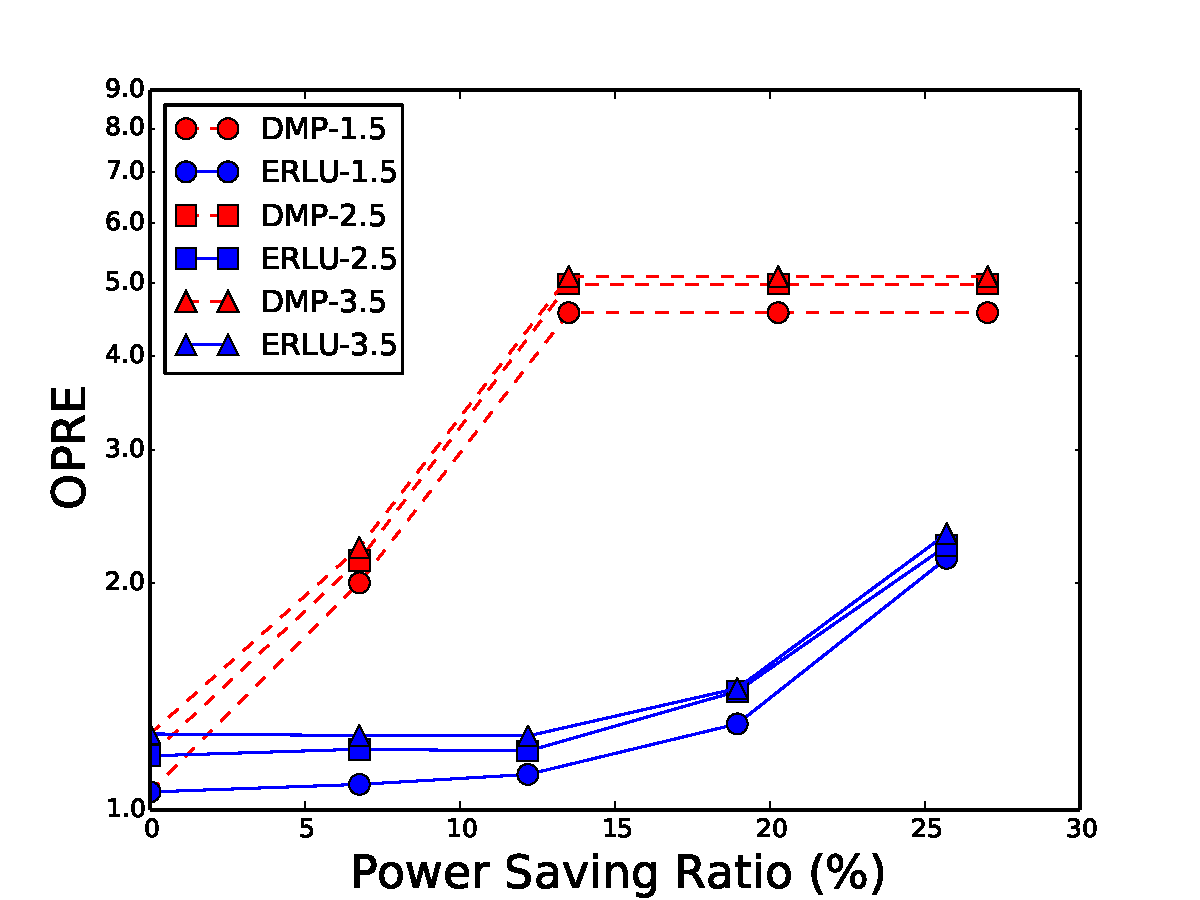
\includegraphics[width=6cm]{opr_with_power_abilene}}
\subfloat{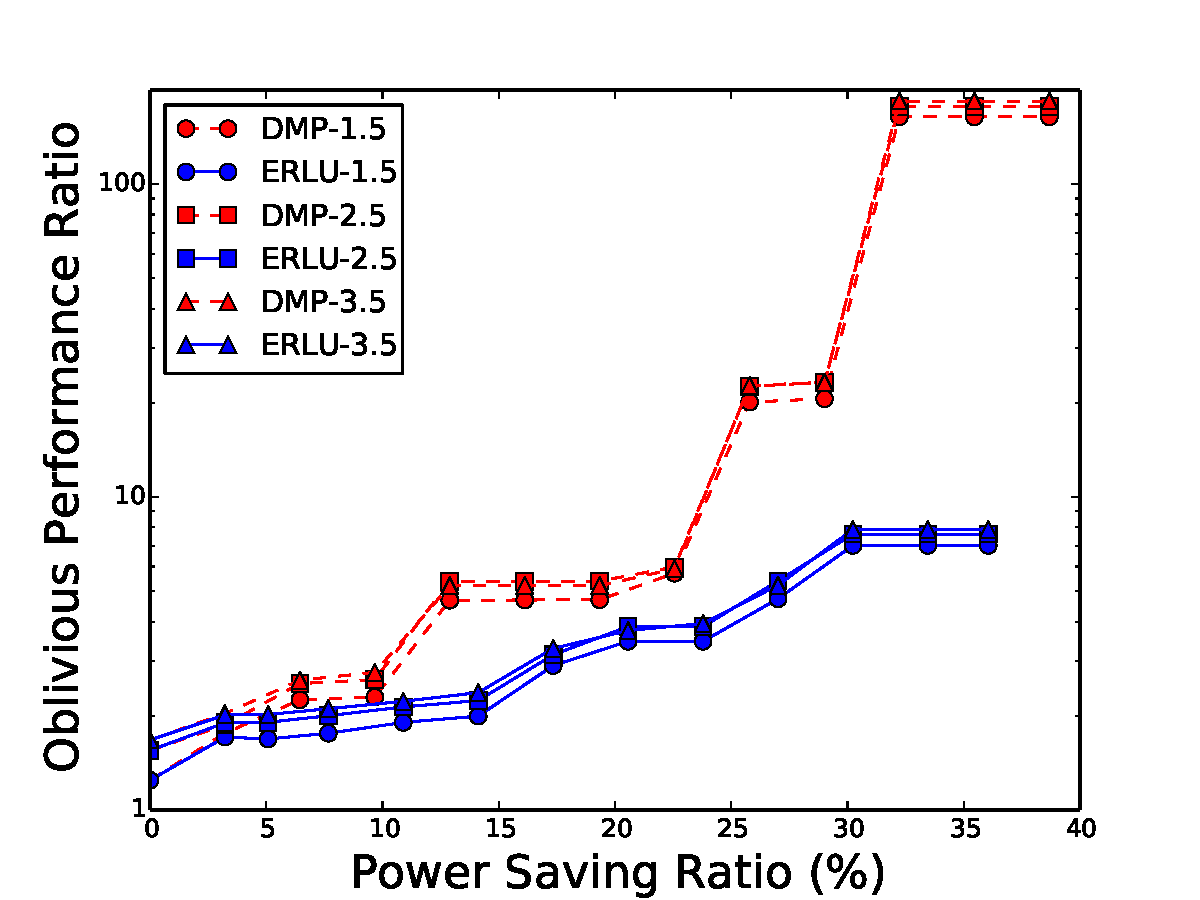
\includegraphics[width=6cm]{opr_with_power_geant}}
\subfloat{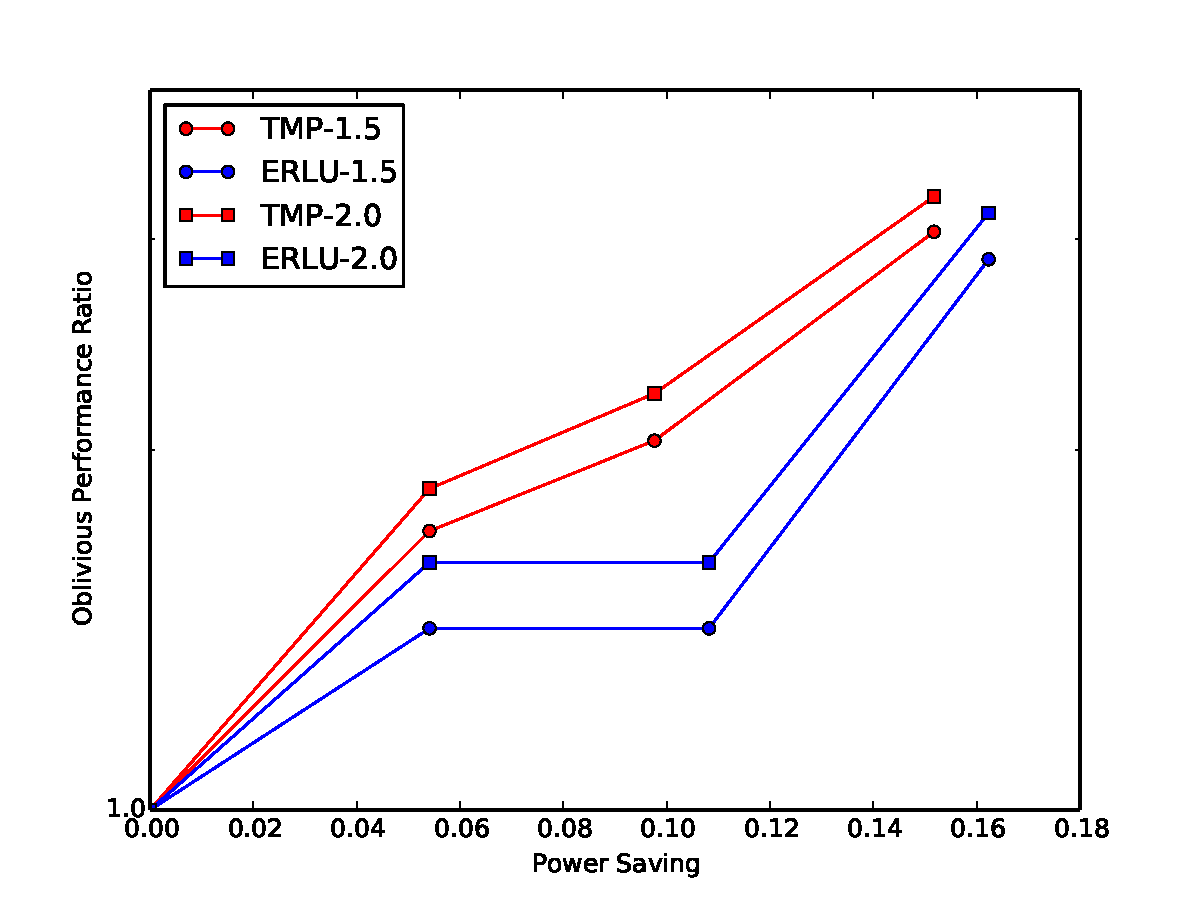
\includegraphics[width=6cm]{opr_with_power_cernet2}}
\caption{OPRE versus TMs: (a). Abilene, (b). Geant, (c). Cernet2}
\label{figure_opr_with_power}
\vspace*{0.1in}
\end{figure*}

\begin{figure*}[!t]
\centering
\vspace*{0.1in}
\subfloat{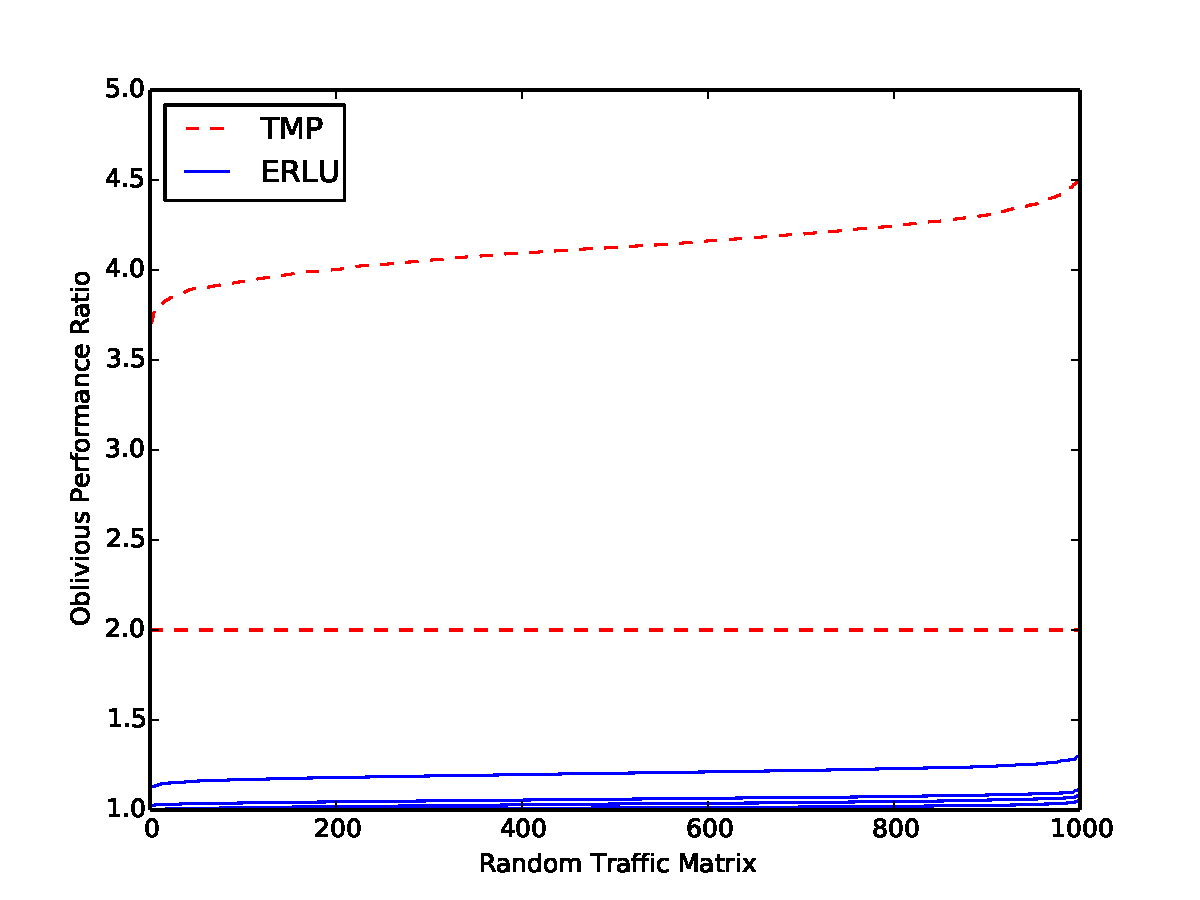
\includegraphics[width=6cm]{exp2_sort_abilene}}
\subfloat{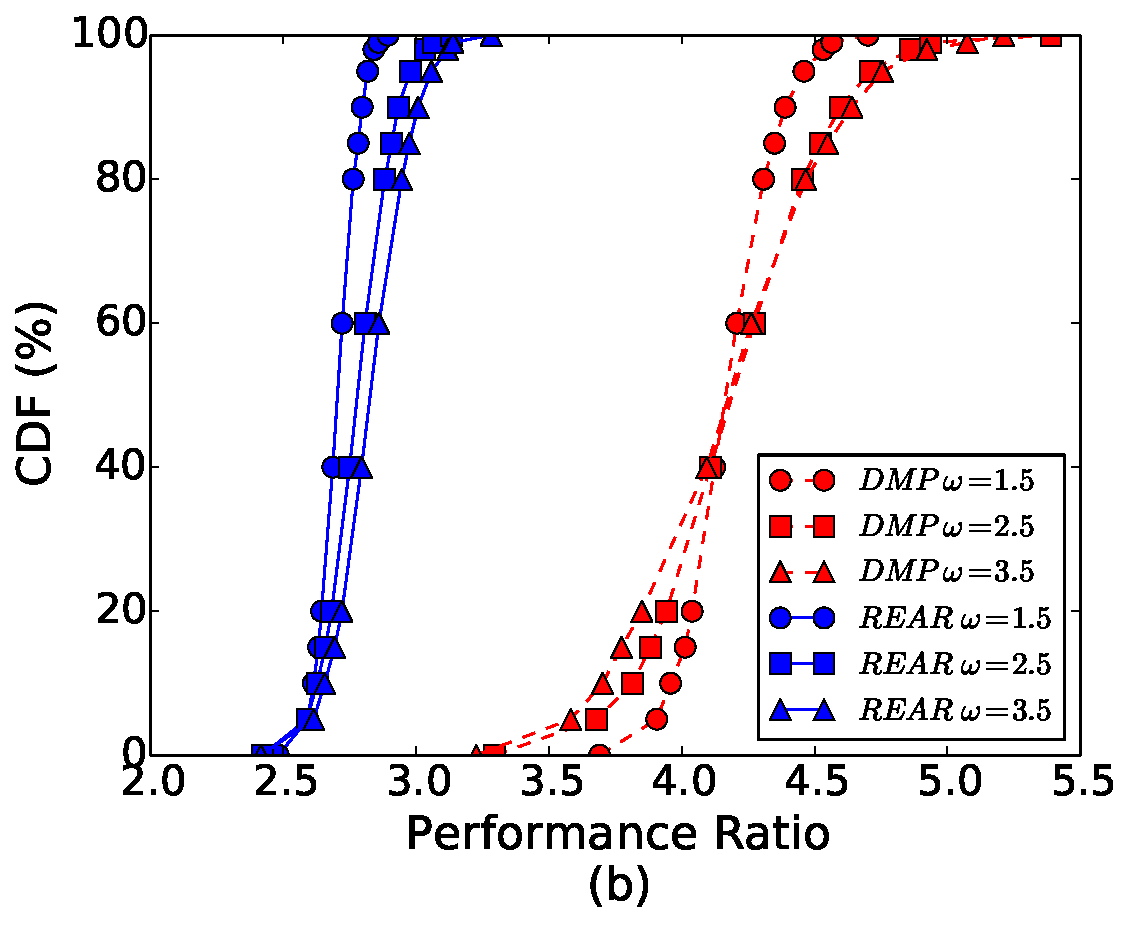
\includegraphics[width=6cm]{exp2_sort_geant}}
\subfloat{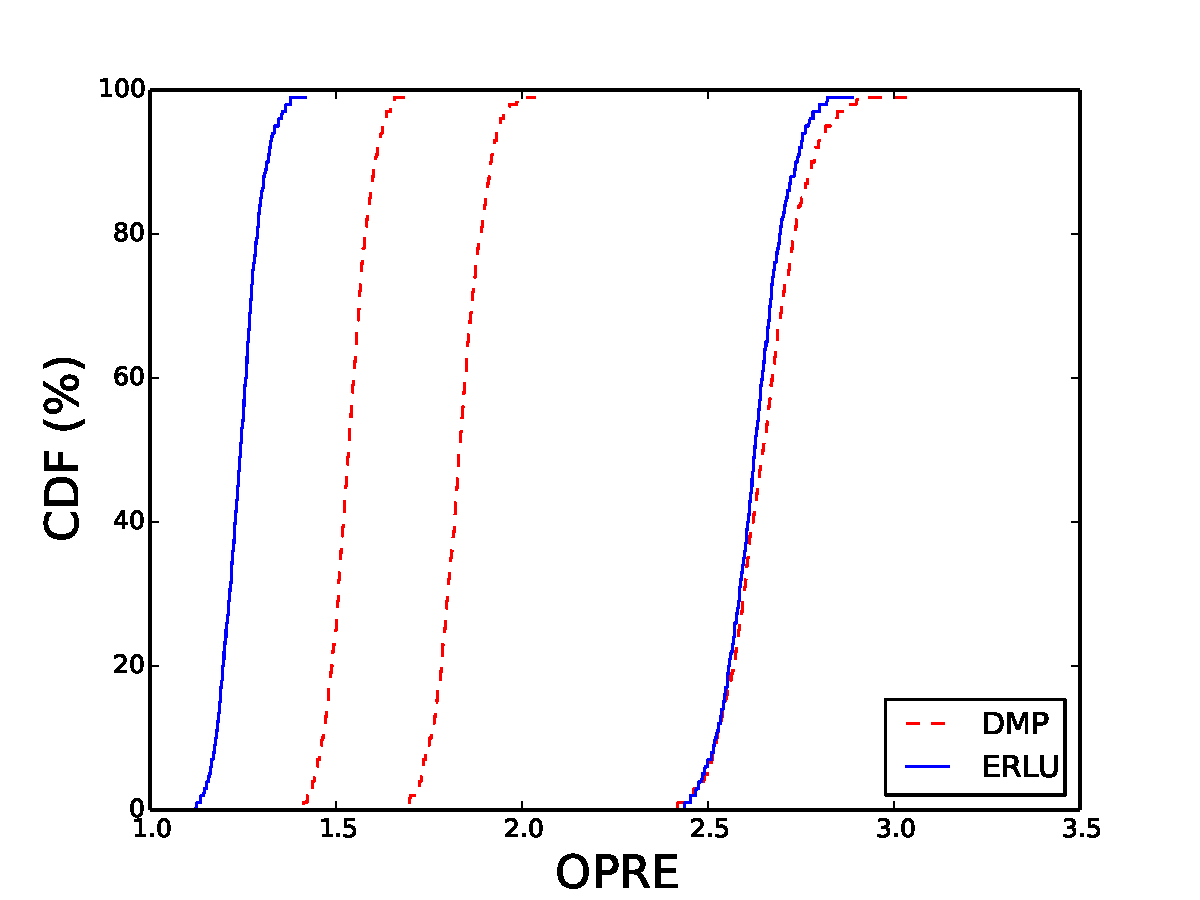
\includegraphics[width=6cm]{exp2_sort_cernet2}}
\caption{OPRE versus Power Saving: (a). Abilene with 4 links removed (b). Geant with 6 links removed (c). Cernet2 with 2 links removed}
\label{figure_exp2_sort}
\vspace*{0.1in}
\end{figure*}


\section{Performance Evaluation}
\label{performance_evaluation}

We evaluate the REAR approach by simulations on three real-world network topologies, including Abilene \cite{networking:abilene}, Geant \cite{networking:geant}, and CERNET2 \cite{networking:cernet2}. The numbers of nodes and links of the topologies are listed in Table \ref{table_topology}. The traffic matrices we used in our simulations are generated as follows. We first generate a baseline traffic matrix using the gravity model \cite{networking:gravity}, where the baseline traffic demand $d_{ab}$ is proportional to their total capacity. Then, the traffic demand is generated randomly in the range from $d_{ab}/\omega$ to $d_{ab}\omega$, where $\omega \geq 1$ is a margin factor used to control the fluctuation range of the traffic. We generate 1000 random TMs for each topology with each $\omega$. The power consumption of different line cards is set as constant in the simulations, as shown in Table \ref{table_line_card_power_consumption}, following \cite{networking:greente}.

\begin{table}[h]
\label{table_topology}
\renewcommand{\arraystretch}{1}
\caption{Topologies}
\label{three topologies}
\centering
\begin{tabular}{|c|c|c|c|}
\hline
\bfseries Topology & \bfseries Nodes & \bfseries Links & \bfseries Links can be Removed \\
\hline
Abilene & 12 & 15 & 4 \\
\hline
Geant & 23 & 37 & 15 \\
\hline
Cernet2 & 20 & 22 & 3 \\
\hline
\end{tabular}
\end{table}

For comparison, we simulate a recent energy efficient routing approach, namely DMP \cite{networking:dmp}, which also does not use the TMs as inputs. DMP always selects the most power-hungry links to switch into off/sleep mode, and can achieve a large power saving ratio, but does not consider routing robustness. We evaluate the OPRE and its distribution, the power saving ratio, and the path stretch of the approaches.

\begin{table}[h]
\label{table_line_card_power_consumption}
\renewcommand{\arraystretch}{1}
\caption{Line Card Power Consumption}
\label{power model}
\centering
\begin{tabular}{|c|c|c|}
\hline
\bfseries Line-Card & \bfseries Speed(Mbps) & \bfseries Power(Watts) \\
\hline
1-Port OC3 & 155.52 & 60 \\
\hline
8-Port OC3 & 1244.16 & 100 \\
\hline
1-Port OC48 & 2488.32 & 140 \\
\hline
1-Port OC192 & 9953.28 & 174 \\
\hline
\end{tabular}
\end{table}

\begin{figure*}[!t]
\centering
\vspace*{0.1in}
\subfloat{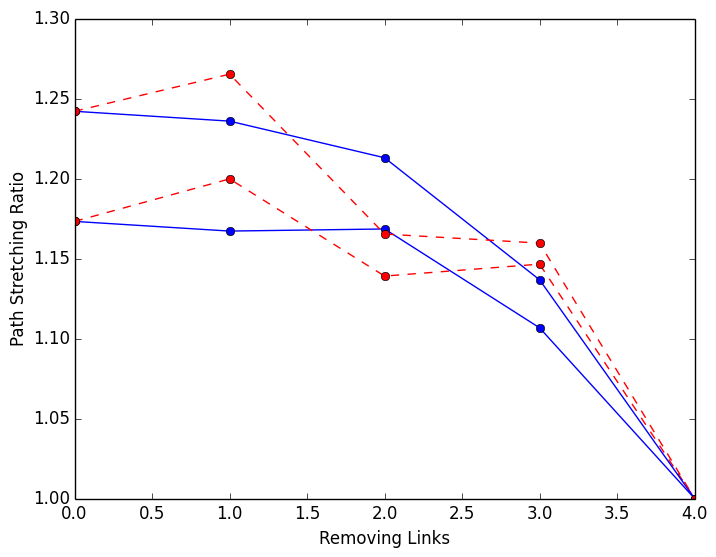
\includegraphics[width=6cm]{exp4_path_abilene}}
\subfloat{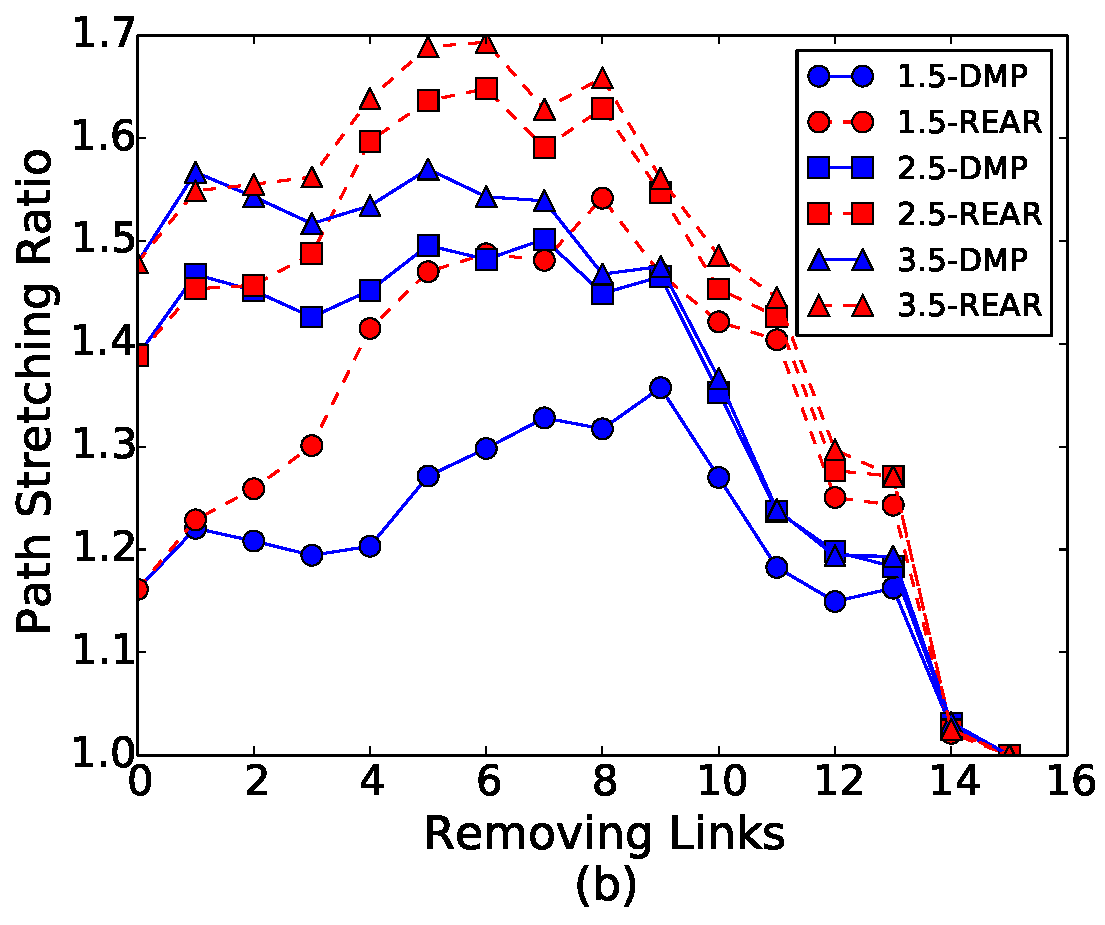
\includegraphics[width=6cm]{exp4_path_geant}}
\subfloat{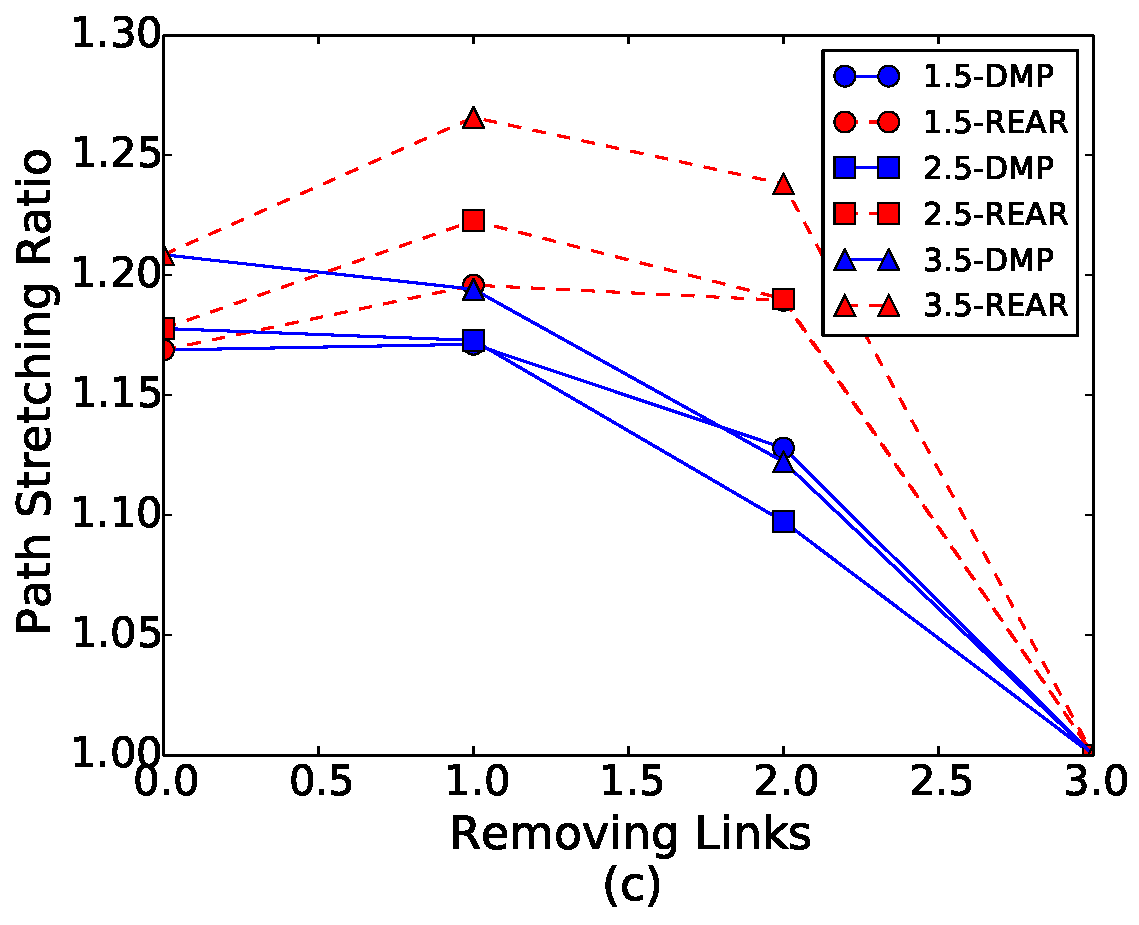
\includegraphics[width=6cm]{exp4_path_cernet2}}
\caption{Path Stretching: (a). Abilene, (b). Geant, (c). Cernet2}
\label{figure_exp4_path}
\vspace*{0.1in}
\end{figure*}

\subsection{OPRE versus Power Saving}
Fig. \ref{figure_opr_with_power} (a) shows the OPRE as a function of power saving ratio $\theta$, in the Abilene topology. We see that the OPRE increases when more power is saved.
This is not surprising because the routing becomes less robust when more links are switched into off/sleep mode. Our REAR has an OPRE ranging from 
1.06 to 2.32, which is much less than the results of DMP. This is because REAR takes routing robustness into consideration when it prunes 
links and computes routing. For instance, when $\omega = 3.5$ and 25\% power is saved, the OPRE of REAR is 2.32, while the OPRE of DMP is 5.09. 
This implies that REAR is more robust against traffic uncertainty. We also see that a larger $\omega$ results in a larger OPRE, because 
the traffic volume fluctuates in a wider range. For instance, when $\omega$ increases from 1.5 to 3.5, the OPRE of REAR increases about 
0.17, while the OPRE of DMP increases about 0.53.

Similar results are showed in Fig. \ref{figure_opr_with_power} (b) and (c), namely in Geant and Cernet2 topology. In Geant, we see that OPRE sacle with a wider range both
in DMP and REAR, it is because Geant is much larger than other topologies, when removing too much links, the network will suffer from more 
serious congestion. In Cernet2, Although REAR is better than DMP, the difference is marginal when achieved a large $\theta$. It can be explained
by the density of links, REAR obtains a better performance in dense topology because it will have more choices.


\subsection{OPRE versus Margin}
Fig. \ref{figure_exp2_sort} (a) shows the amount of TMs as a cumulative distribution function (CDF) of OPRE, when remove 4 links in Abilene topology. We see that the curves of
DMP are right of REAR, means REAR always have lower OPRE whatever TMs is. It is consistent with Fig. \ref{figure_opr_with_power} (a). We also observe that our REAR has
more concentrated curves, means REAR have the almost same performance when TM changes, it is because REAR remove the less `important' link from 
topology and the left topology is more robust for TMs than DMP. For instance, REAR ranges from 1.74 to 2.32 while DMP range from 2.97 to 5.09 
when $\omega = 3.5$. Also we can see that curve become smooth when $\omega$ increases, it is because the TMs range from wider scope, and the OPRE
may achieved wider scope too. However we see that whatever $\omega$ is, the center of the curve are almost the same postion. It is because 
we only change the margin $\omega$ rather than the base TM, so the medial value will not changes apparently.


Fig. \ref{figure_exp2_sort} (b) shows the amount of TMs as a CDF of OPRE when remove 6 links in Geant, and Fig. \ref{figure_exp2_sort} (c) shows the situation when remove 2 links in Cernet2.
Similar results are showed in them, however both the centers of REAR curve in Fig. \ref{figure_exp2_sort} (b) and DMP in Fig. \ref{figure_exp2_sort} (c) are not at the same postion 
when $\omega$ changes. The reasons are two-folds, firstly the curves is drawn by sampling from origin data so the center of curve may not the real 
center. On the other hand, we calculate the distance of centers over the scope of OPRE, respectively 0.9\% for REAR in Geant and 0.1\% for DMP in Cernet2,
so it is obvious that from sight of the scope of OPRE, the center of curves are the same `postion'.



\subsection{Path Stretching}
Fig. \ref{figure_exp4_path} (a) shows the path stretching ratio (PSR) as a function of the number of removed links in Abilene topology. We see that PSR will 
equal to 1 when maximum number of links are removed. It is because when the topology reduces to a spanning tree, the routing between two 
vertices become unique, namely each path is the shortest path. Our REAR has an worst PSR value of 1.30, better than 1.36 in DMP, when 
remove 1 link and $\omega = 3.5$. We observe that when remove more than 1 link, the DMP is even better than REAR sometimes. This is 
because both REAR and DMP implement our RRP algorihtm for adjusting routing, and in RRP we always choose the routing path from k-shortest 
paths for the traffic on the removed link, which make the PSR little as possible. We also see that a larger $\omega$ results in a 
larger PSR, and reduces to 1 as explained above, because the demand-oblivious routing is computed based on $\omega$, when $\omega$ increases
the routing will find much more paths for avoiding sudden traffic demand, which makes the PSR increases. For example, when $\omega$ increases
from 1.5 to 3.5, the PSR of REAR increases about 0.08, while the PSR of DMP increasess about 0.14.

Fig. \ref{figure_exp4_path} (b) and Fig. \ref{figure_exp4_path} (c) show the similar results in Geant and Cernet2, while our REAR is always better than DMP. For instance, REAR
have the worst PSR of 1.35 and DMP is 1.54 when $\omega = 1.5$ in Geant, REAR have the worst PSR of 1.20 and DMP is 1.27 when $\omega = 3.5$


\section{Conclusion}
\label{conclusion}
The conclusion goes here.

\begin{thebibliography}{1}

\bibitem{networking:designing}
J. Carter and K. Rajamani, ``Designing Energy-Efficient Servers and Data Centers," Computer, 2010.

\bibitem{networking:active}
S. Avallone, G. Ventre. ``Energy efficient online routing of flows with additive constraints." Computer Networks, 2012.

\bibitem{networking:greente}
M. Zhang, C. Yi, B. Liu, et al. ``GreenTE: Power-Aware Traffic Engineering," in Proc. of IEEE ICNP, October 2010.

\bibitem{networking:car}
A. Cianfrani, V. Eramo, M. Listanti, and M. Polverini, ``An OSPF enhancement for energy saving in IP networks," in IEEE INFOCOM Workshop on Green Communications and Networking, April 2011.

\bibitem{networking:grida}
A. P. Bianzino, L. Chiaraviglio, M. Mellia, et al. ``GRiDA: GReen Distributed Algorithm for energy-efficient IP backbone networks," Computer Networks, 2012.

\bibitem{networking:greenfrr}
Y. Yang, M. Xu, Q. Li. ``Towards fast rerouting-based energy efficient routing," Computer Networks, 2014.

\bibitem{networking:oblivious}
D. Applegate and E. Cohen, ``Making Intra-Domain Routing Robust to Changing and Uncertain Traffic Demands: Understanding Fundamental Tradeoffs," in Proceedings of ACM SIGCOMM ’03, Karlsruhe, Germany, August 2003.

\bibitem{networking:lp}
O. Goldschmidt. ``ISP Backbone Traffic Inference Methods to Support Traffic Engineering," In Internet Statistics and Metrics Analysis (ISMA) Workshop, San Diego, CA, December 2000.

\bibitem{networking:bayesian}
C. Tebaldi and M. West. ``Bayesian Inference of Network Traffic Using Link Count Data," J. of the American Statistical Association, June 1998.

\bibitem{networking:time}
J. Cao, D. Davis, S. Vander Weil, and B. Yu. ``Time-Varying Network Tomography," J. of the American Statistical Association, 2000.

\bibitem{networking:minimize}
Harald R\"{a}cke. ``Minimizing congestion in general networks," In Proceedings of the 43rd IEEE Symposium on Foundations of Computer Science (FOCS), 2002. Co-Winner of Best Paper Award.

\bibitem{networking:polynomial}
Y. Azar, E. Cohen, A. Fiat, H. Kaplan, and H. R ̈acke. ``Optimal oblivious routing in polynomial time," In Proceedings of the 35th ACM Symposium on the Theory of Computing, 2003.

\bibitem{networking:gravity}
M.Roughan, A.Greenberg, C.Kalmanek, M.Rumsewicz, J.Yates, and Y.Zhang. ``Experience in measuring backbone traffic variability: models, metrics, measurements, and meaning," InProceedings of the 2nd Internet Measurement Workshop. ACM, 2002

\bibitem{networking:dmp}
A.P. Bianzino, L. Chiaraviglio, M. Mellia, ``Distributed algorithms for green IP networks," in: IEEE INFOCOM Workshop on Green Networking and Smart Grid, 2012

\bibitem{networking:hopbyhop}
C. Hou, F. Zhang, A. F. Anta, L. Wang, and Z. Liu. ``A Hopby-hop Energy Efficient Distributed Routing Scheme," in Proc. of Greenmetrics Workshop, 2013.

\bibitem{networking:yens}
Yen, Jin Y. ``Finding the k Shortest Loopless Paths in a Network," Management Science 17 (11), 1971

\bibitem{networking:abilene}
``Abilene Core Topology," [Online], Available: https://itservices.
stanford.edu/service/network/internet2/abilene

\bibitem{networking:geant}
``Network Topology," [Online], Available: http://geant3.archive.ge
ant.net/Network/NetworkTopology/pages/home.aspx

\bibitem{networking:cernet2}
``Cernet2 Topology," [Online], Available: http://www.edu.cn/20060111
/3170220.shtml

\end{thebibliography}

\appendices

\section{Proof of Theorem 3}
\begin{proof}
Fig. \ref{figure_circle_and_clique} shows the 6-nodes cycle and clique topologies. We label three links $l_{ab}$, $l_{cd}$ and $l_{ef}$
for our proof, let $cap_{ab}$, $cap_{cd}$ and $cap_{ef}$ be their link capacities. Now a arbitrary traffic
comes, we compute the optimal routing and forward the demand on the topologies, let $dem_{ab}$, $dem_{cd}$
and $dem_{ef}$ be the traffic on each link. Without loss of generality, we say the link $l_{ab}$ is the
bottleneck, namely the link with MLUR.


Now let's consider the robust routing. When the routing changes, the traffic on each link also changes.
We image a simple situation, just forward the traffic from one link to another path base on the optimal
routing, and the link utilization of links on the path will increase, and accordingly the link
utilization of former link will reduce to 0. Obviously, the routing must have a worse performance than
the optimal robust routing, so its upper bound also is the bound of minimum OPRE.


\begin{figure}[!t]
\centering
\vspace*{0.1in}
\subfloat[Circle]{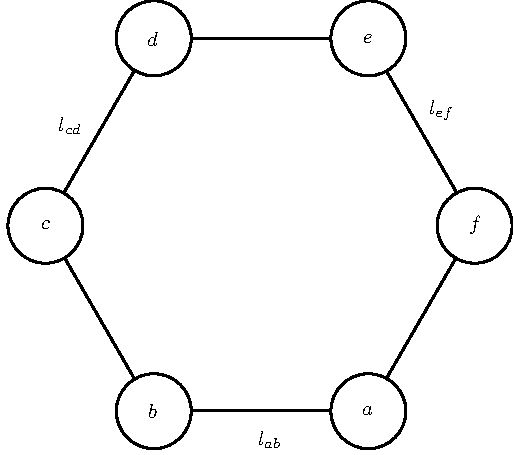
\includegraphics[width=4cm]{circle}
\label{subfiga}}
\hfill
\subfloat[Clique]{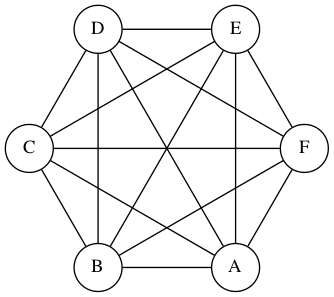
\includegraphics[width=4cm]{clique}
\label{subfigb}}
\caption{Circle and Clique topology of 6 nodes}
\label{figure_circle_and_clique}
\vspace*{0.1in}
\end{figure}

For Case \Rmnum{1}.\Rmnum{1}, the adjusted link may be $l_{cd}$, the new bottleneck still be $l_{ab}$.
The traffic on $l_{ab}$ is increased by the origin traffic on link $l_{cd}$, So we compute OPRE by:

\begin{equation}
\label{equation_A_1_1_1}
\frac {\frac{dem_{ab} + dem_{cd}}{cap_{ab}}} {\frac{dem_{ab}}{cap_{ab}}} = 1 + \frac{dem_{cd}}{dem_{ab}}
\end{equation}

Because the old bottleneck is $l_{ab}$, so we have inequation:

\begin{equation}
\label{inequation_A_1_1_2}
\frac {dem_{cd}} {cap_{cd}} < \frac {dem_{ab}} {cap_{ab}}
\end{equation}

From Ineq. (\ref{inequation_A_1_1_2}) we get:

\begin{equation}
\label{inequation_A_1_1_3}
\frac {dem_{cd}} {dem_{ab}} < \frac {cap_{cd}} {cap_{ab}}
\end{equation}

So we have OPRE in Case \Rmnum{1}.\Rmnum{1} combined by Eq. (\ref{equation_A_1_1_1}) and Ineq. (\ref{inequation_A_1_1_3}):

\begin{equation}
\label{inequation_A_1_1_result}
1 + \frac {dem_{cd}} {dem_{ab}} < 1 + \frac {cap_{cd}} {cap_{ab}}
\end{equation}

For Case \Rmnum{1}.\Rmnum{2}, the adjusted link also be $l_{cd}$, but the new bottleneck may be $l_{ef}$.
Computing the OPRE similar as above:

\begin{equation}
\label{equation_A_1_2_1}
\frac {\frac{dem_{ef} + dem_{cd}}{cap_{ef}}} {\frac{dem_{ab}}{cap_{ab}}} =
\frac {dem_{ef} * cap_{ab}}{dem_{ab} * cap_{ef}} + \frac {dem_{cd} * cap_{ab}}{dem_{ab} * cap_{ef}}
\end{equation}

Because the old bottleneck is $l_{ab}$, so we have Ineq. (\ref{inequation_A_1_1_2}) and :

\begin{equation}
\label{inequation_A_1_2_2}
\frac {dem_{ef}} {cap_{ef}} < \frac {dem_{ab}} {cap_{ab}}
\end{equation}

So we get inequation from Ineq. (\ref{inequation_A_1_2_2}):

\begin{equation}
\label{inequation_A_1_2_3}
\frac {dem_{ef} * cap_{ab}} {dem_{ab} * cap_{ef}} < 1
\end{equation}

Also from Ineq. (\ref{inequation_A_1_1_2}) we have :

\begin{equation}
\label{inequation_A_1_2_4}
\frac {dem_{cd} * cap_{ab}} {dem_{ab}} < cap_{cd}
\end{equation}

Combine Eq. (\ref{equation_A_1_2_1}), Ineq. (\ref{inequation_A_1_2_3}) and Ineq. (\ref{inequation_A_1_2_4}), we have OPRE in Case \Rmnum{1}.\Rmnum{2}:

\begin{equation}
\label{inequation_A_1_2_result}
\frac {dem_{ef} * cap_{ab}}{dem_{ab} * cap_{ef}} + \frac {dem_{cd} * cap_{ab}}{dem_{ab} * cap_{ef}}
< 1 + \frac {cap_{cd}}{cap_{ef}}
\end{equation}

For Case \Rmnum{2}, the adjusted link may be $l_{ab}$, namely the old bottleneck link, the new bottleneck
maybe $l_{ef}$. Computing the OPRE similar as above:

\begin{equation}
\label{equation_A_2_1}
\frac {\frac{dem_{ef} + dem_{ab}}{cap_{ef}}} {\frac{dem_{ab}}{cap_{ab}}} =
\frac {dem_{ef} * cap_{ab}}{dem_{ab} * cap_{ef}} + \frac{cap_{ab}}{cap_{ef}}
\end{equation}

Becuase the old bottleneck has the maximum link utilization, so combine Ineq. (\ref{inequation_A_1_2_3}) and Eq. (\ref{equation_A_2_1}) we obtain OPRE in Case
\Rmnum{2}:

\begin{equation}
\label{inequation_A_2_result}
\frac {dem_{ef} * cap_{ab}}{dem_{ab} * cap_{ef}} + \frac{cap_{ab}}{cap_{ef}} < 1 + \frac{cap_{ab}}{cap_{ef}}
\end{equation}


To sum up, we have inequation from Ineq. (\ref{inequation_A_1_1_result}), Ineq. (\ref{inequation_A_1_2_result}) and Ineq. (\ref{inequation_A_2_result}):

\begin{equation}
\label{inequation_A_result}
1 + \max \{\frac{cap_{cd}}{cap_{ab}}, \frac{cap_{cd}}{cap_{ef}}, \frac{cap_{ab}}{cap_{ef}} \} < 1 + \frac{\max_{l \in E} cap_{l}}{\min_{l \in E} cap_{l}}
\end{equation}

\end{proof}

\section{Proof of Theorem 4}
\begin{proof}
The spanning tree of circle is the topology which lose one link. In Appendix. A, when we consider the robust routing, we adjust the traffic
on one link to another path, it is similar that we switch off the link and forward the traffic to some other path. The complete proof is
almost the same with Appendix. A.
\end{proof}

\section{Proof of Theorem 5}
\begin{proof}
Every link in the spanning tree will split the graph to two components, the flow between them must need trace this link.
we say the bottleneck link is $l_{ab}$ for optimal routing on the origin topology, and let $l_{ef}$ be the bottleneck link for
the robust routing on the spanning tree. Other symbols are consistent with Appendix. A. So we have OPRE:

\begin{equation}
\label{equation_C_1}
    \frac{\frac{\sum_{(i,j) \in E} dem_{ij}}{cap_{ef}}}{\frac{dem_{ab}}{cap_{ab}}} = \frac{cap_{ab}}{cap_{ef}} \sum_{(i,j) \in E} \frac{dem_{ij}}{dem_{ab}}
\end{equation}

Because the $l_{ab}$ is the bottleneck link, we have:

\begin{equation}
\label{ineqaution_C_2}
    \frac{dem_{ij}}{cap_{ij}} < \frac{dem_{ab}}{cap_{ab}}, \forall (i,j) \in E
\end{equation}

\begin{equation}
\label{ineqaution_C_3}
    \frac{dem_{ij} * cap_{ab}}{dem_{ab}} < cap_{ij}, \forall (i,j) \in E
\end{equation}

So we have OPRE:

\begin{equation}
\label{ineqaution_C_4}
    \frac{cap_{ab}}{cap_{ef}} \sum_{(i,j) \in E} \frac{dem_{ij}}{dem_{ab}} < \sum_{(i,j) \in E} \frac{cap_{ij}}{cap_{ef}}
\end{equation}

And we know that, the amount of $l_{ij}$ between two parts must less than $\frac{n^2}{2}$, so OPRE must lower than:

\begin{equation}
\label{ineqaution_C_result}
    \sum_{(i,j) \in E} \frac{cap_{ij}}{cap_{ef}} < \frac{n^2}{2} \frac{\max_{l \in E} cap_l}{\min_{l \in E} cap_l}
\end{equation}

\end{proof}

% that's all folks
\end{document}



























